\documentclass{standalone}
\usepackage{tikz}
\usetikzlibrary{patterns, positioning}

\begin{document}
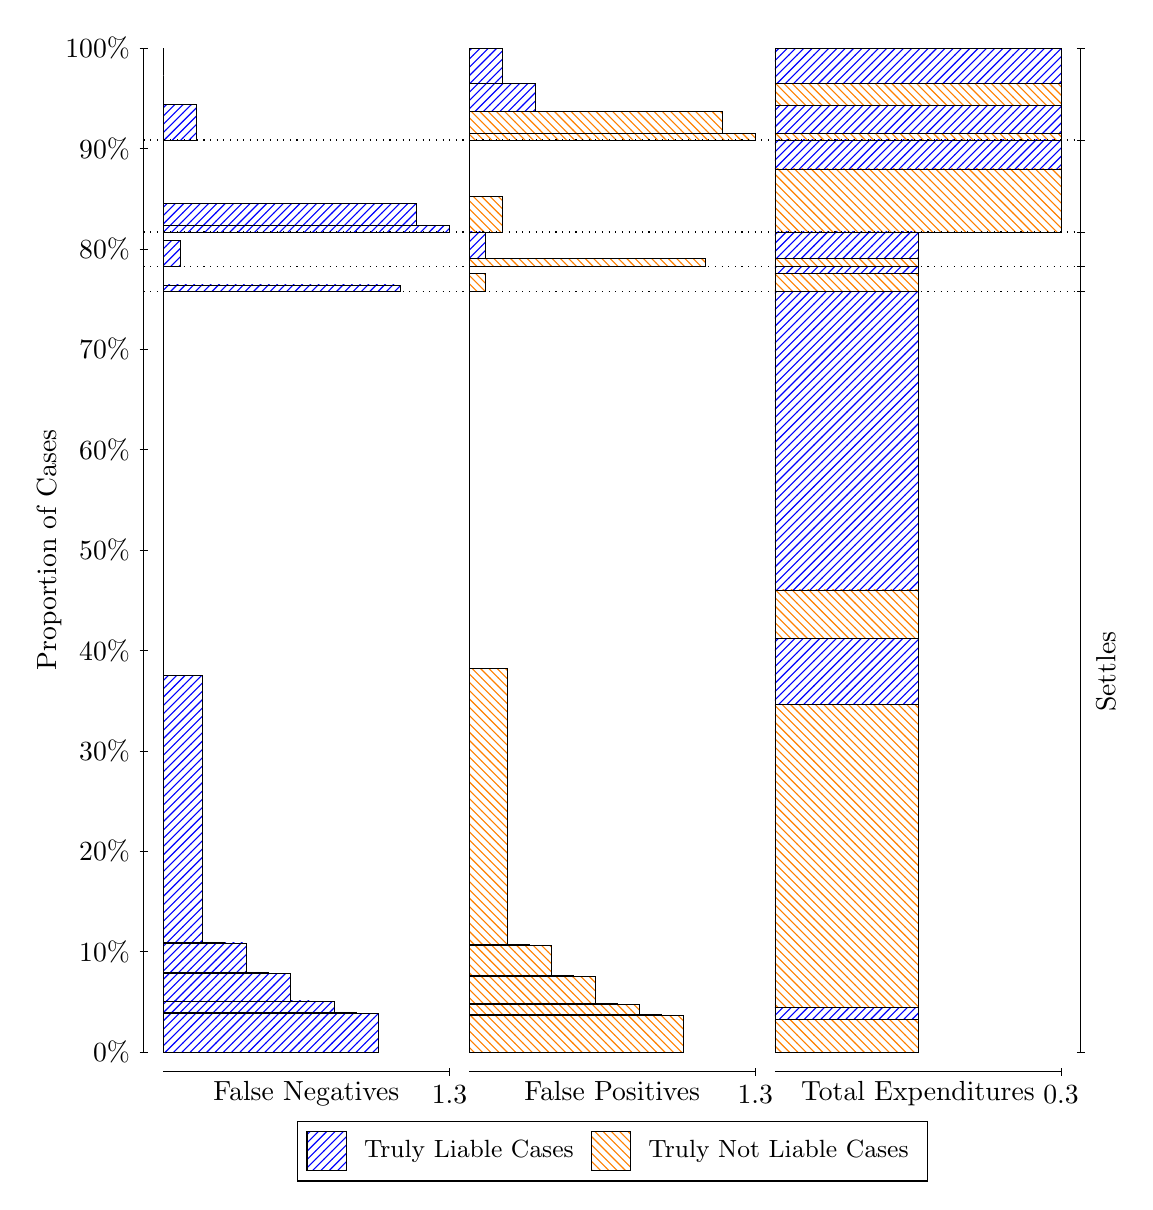
\begin{tikzpicture}
\draw[black, very thin] (1.5,1.75) -- (1.5,14.5);
\node[rotate=90, anchor=center] at (0.3, 8.125) {Proportion of Cases};
\draw[black, very thin] (1.45,1.75) -- (1.55,1.75);
\node[anchor=east] at (1.45, 1.75) {0\%};
\draw[black, very thin] (1.45,3.025) -- (1.55,3.025);
\node[anchor=east] at (1.45, 3.025) {10\%};
\draw[black, very thin] (1.45,4.3) -- (1.55,4.3);
\node[anchor=east] at (1.45, 4.3) {20\%};
\draw[black, very thin] (1.45,5.575) -- (1.55,5.575);
\node[anchor=east] at (1.45, 5.575) {30\%};
\draw[black, very thin] (1.45,6.85) -- (1.55,6.85);
\node[anchor=east] at (1.45, 6.85) {40\%};
\draw[black, very thin] (1.45,8.125) -- (1.55,8.125);
\node[anchor=east] at (1.45, 8.125) {50\%};
\draw[black, very thin] (1.45,9.4) -- (1.55,9.4);
\node[anchor=east] at (1.45, 9.4) {60\%};
\draw[black, very thin] (1.45,10.675) -- (1.55,10.675);
\node[anchor=east] at (1.45, 10.675) {70\%};
\draw[black, very thin] (1.45,11.95) -- (1.55,11.95);
\node[anchor=east] at (1.45, 11.95) {80\%};
\draw[black, very thin] (1.45,13.225) -- (1.55,13.225);
\node[anchor=east] at (1.45, 13.225) {90\%};
\draw[black, very thin] (1.45,14.5) -- (1.55,14.5);
\node[anchor=east] at (1.45, 14.5) {100\%};

\draw[black, very thin] (13.4,1.75) -- (13.4,14.5);
\draw[black, very thin] (13.35,1.75) -- (13.45,1.75);
\node[anchor=west] at (13.35, 1.75) {};
\draw[black, very thin] (13.35,11.408) -- (13.45,11.408);
\node[anchor=west] at (13.35, 11.408) {};
\draw[black, very thin] (13.35,11.722) -- (13.45,11.722);
\node[anchor=west] at (13.35, 11.722) {};
\draw[black, very thin] (13.35,12.164) -- (13.45,12.164);
\node[anchor=west] at (13.35, 12.164) {};
\draw[black, very thin] (13.35,13.332) -- (13.45,13.332);
\node[anchor=west] at (13.35, 13.332) {};
\draw[black, very thin] (13.35,14.5) -- (13.45,14.5);
\node[anchor=west] at (13.35, 14.5) {};

\draw[black, very thin, pattern color=blue, pattern=north east lines] (1.75,1.75) rectangle (4.475,2.2437);
\draw[black, very thin, pattern color=blue, pattern=north east lines] (1.75,2.2437) rectangle (4.1955,2.2502);
\draw[black, very thin, pattern color=blue, pattern=north east lines] (1.75,2.2502) rectangle (3.916,2.3892);
\draw[black, very thin, pattern color=blue, pattern=north east lines] (1.75,2.3892) rectangle (3.6365,2.3983);
\draw[black, very thin, pattern color=blue, pattern=north east lines] (1.75,2.3983) rectangle (3.3571,2.7455);
\draw[black, very thin, pattern color=blue, pattern=north east lines] (1.75,2.7455) rectangle (3.0776,2.7622);
\draw[black, very thin, pattern color=blue, pattern=north east lines] (1.75,2.7622) rectangle (2.7981,3.1364);
\draw[black, very thin, pattern color=blue, pattern=north east lines] (1.75,3.1364) rectangle (2.5186,3.1445);
\draw[black, very thin, pattern color=blue, pattern=north east lines] (1.75,3.1445) rectangle (2.2391,6.5349);
\draw[black, very thin, pattern color=orange, pattern=north west lines] (1.75,6.5349) rectangle (1.75,11.408);
\draw[black, very thin, pattern color=blue, pattern=north east lines] (1.75,11.408) rectangle (4.7545,11.492);
\draw[black, very thin, pattern color=orange, pattern=north west lines] (1.75,11.492) rectangle (1.75,11.722);
\draw[black, very thin, pattern color=blue, pattern=north east lines] (1.75,11.722) rectangle (1.9596,12.06);
\draw[black, very thin, pattern color=orange, pattern=north west lines] (1.75,12.06) rectangle (1.75,12.164);
\draw[black, very thin, pattern color=blue, pattern=north east lines] (1.75,12.164) rectangle (5.3833,12.249);
\draw[black, very thin, pattern color=blue, pattern=north east lines] (1.75,12.249) rectangle (4.9641,12.53);
\draw[black, very thin, pattern color=orange, pattern=north west lines] (1.75,12.53) rectangle (1.75,13.332);
\draw[black, very thin, pattern color=blue, pattern=north east lines] (1.75,13.332) rectangle (2.1692,13.784);
\draw[black, very thin, pattern color=orange, pattern=north west lines] (1.75,13.784) rectangle (1.75,14.15);
\draw[black, very thin, pattern color=blue, pattern=north east lines] (1.75,14.15) rectangle (1.75,14.5);
\draw[black, very thin, pattern color=orange, pattern=north west lines] (5.6333,1.75) rectangle (8.3583,2.2192);
\draw[black, very thin, pattern color=orange, pattern=north west lines] (5.6333,2.2192) rectangle (8.0788,2.2225);
\draw[black, very thin, pattern color=orange, pattern=north west lines] (5.6333,2.2225) rectangle (7.7994,2.3554);
\draw[black, very thin, pattern color=orange, pattern=north west lines] (5.6333,2.3554) rectangle (7.5199,2.3634);
\draw[black, very thin, pattern color=orange, pattern=north west lines] (5.6333,2.3634) rectangle (7.2404,2.7065);
\draw[black, very thin, pattern color=orange, pattern=north west lines] (5.6333,2.7065) rectangle (6.9609,2.7104);
\draw[black, very thin, pattern color=orange, pattern=north west lines] (5.6333,2.7104) rectangle (6.9609,2.7219);
\draw[black, very thin, pattern color=orange, pattern=north west lines] (5.6333,2.7219) rectangle (6.6814,3.105);
\draw[black, very thin, pattern color=orange, pattern=north west lines] (5.6333,3.105) rectangle (6.4019,3.1177);
\draw[black, very thin, pattern color=orange, pattern=north west lines] (5.6333,3.1177) rectangle (6.1224,6.6228);
\draw[black, very thin, pattern color=blue, pattern=north east lines] (5.6333,6.6228) rectangle (5.6333,11.408);
\draw[black, very thin, pattern color=orange, pattern=north west lines] (5.6333,11.408) rectangle (5.8429,11.638);
\draw[black, very thin, pattern color=blue, pattern=north east lines] (5.6333,11.638) rectangle (5.6333,11.722);
\draw[black, very thin, pattern color=orange, pattern=north west lines] (5.6333,11.722) rectangle (8.6378,11.826);
\draw[black, very thin, pattern color=blue, pattern=north east lines] (5.6333,11.826) rectangle (5.8429,12.164);
\draw[black, very thin, pattern color=orange, pattern=north west lines] (5.6333,12.164) rectangle (6.0526,12.616);
\draw[black, very thin, pattern color=orange, pattern=north west lines] (5.6333,12.616) rectangle (5.6333,12.966);
\draw[black, very thin, pattern color=blue, pattern=north east lines] (5.6333,12.966) rectangle (5.6333,13.332);
\draw[black, very thin, pattern color=orange, pattern=north west lines] (5.6333,13.332) rectangle (9.2667,13.417);
\draw[black, very thin, pattern color=orange, pattern=north west lines] (5.6333,13.417) rectangle (8.8474,13.698);
\draw[black, very thin, pattern color=blue, pattern=north east lines] (5.6333,13.698) rectangle (6.4718,14.048);
\draw[black, very thin, pattern color=blue, pattern=north east lines] (5.6333,14.048) rectangle (6.0526,14.5);
\draw[black, very thin, pattern color=orange, pattern=north west lines] (9.5167,1.75) rectangle (11.333,2.1613);
\draw[black, very thin, pattern color=blue, pattern=north east lines] (9.5167,2.1613) rectangle (11.333,2.3159);
\draw[black, very thin, pattern color=orange, pattern=north west lines] (9.5167,2.3159) rectangle (11.333,6.164);
\draw[black, very thin, pattern color=blue, pattern=north east lines] (9.5167,6.164) rectangle (11.333,7.0048);
\draw[black, very thin, pattern color=orange, pattern=north west lines] (9.5167,7.0048) rectangle (11.333,7.6182);
\draw[black, very thin, pattern color=blue, pattern=north east lines] (9.5167,7.6182) rectangle (11.333,11.408);
\draw[black, very thin, pattern color=orange, pattern=north west lines] (9.5167,11.408) rectangle (11.333,11.638);
\draw[black, very thin, pattern color=blue, pattern=north east lines] (9.5167,11.638) rectangle (11.333,11.722);
\draw[black, very thin, pattern color=orange, pattern=north west lines] (9.5167,11.722) rectangle (11.333,11.826);
\draw[black, very thin, pattern color=blue, pattern=north east lines] (9.5167,11.826) rectangle (11.333,12.164);
\draw[black, very thin, pattern color=orange, pattern=north west lines] (9.5167,12.164) rectangle (13.15,12.966);
\draw[black, very thin, pattern color=blue, pattern=north east lines] (9.5167,12.966) rectangle (13.15,13.332);
\draw[black, very thin, pattern color=orange, pattern=north west lines] (9.5167,13.332) rectangle (13.15,13.417);
\draw[black, very thin, pattern color=blue, pattern=north east lines] (9.5167,13.417) rectangle (13.15,13.767);
\draw[black, very thin, pattern color=orange, pattern=north west lines] (9.5167,13.767) rectangle (13.15,14.048);
\draw[black, very thin, pattern color=blue, pattern=north east lines] (9.5167,14.048) rectangle (13.15,14.5);
\draw[black, dotted] (1.5,11.408) -- (13.4,11.408);
\draw[black, dotted] (1.5,11.722) -- (13.4,11.722);
\draw[black, dotted] (1.5,12.164) -- (13.4,12.164);
\draw[black, dotted] (1.5,13.332) -- (13.4,13.332);
\draw[black, very thin] (1.75,1.5) -- (5.3833,1.5);
\node[anchor=north] at (3.5667, 1.5) {False Negatives};
\draw[black, very thin] (5.3833,1.45) -- (5.3833,1.55);
\node[anchor=north] at (5.3833, 1.45) {1.3};

\draw[black, very thin] (5.6333,1.5) -- (9.2667,1.5);
\node[anchor=north] at (7.45, 1.5) {False Positives};
\draw[black, very thin] (9.2667,1.45) -- (9.2667,1.55);
\node[anchor=north] at (9.2667, 1.45) {1.3};

\draw[black, very thin] (9.5167,1.5) -- (13.15,1.5);
\node[anchor=north] at (11.333, 1.5) {Total Expenditures};
\draw[black, very thin] (13.15,1.45) -- (13.15,1.55);
\node[anchor=north] at (13.15, 1.45) {0.3};

\node[black, centered, rotate=90] at (13.72, 6.5788) {Settles};





\draw (7.449999999999999,1.5) node[draw=none] (baseCoordinate) {};
\begin{scope}[align=center]
        \matrix[scale=0.5, draw=black, below=0.5cm of baseCoordinate, nodes={draw}, column sep=0.1cm]{
            \node[rectangle, draw, minimum width=0.5cm, minimum height=0.5cm, pattern=north east lines, pattern color=blue] {}; &
            \node[draw=none, font=\small] (B) {Truly Liable Cases}; &
            \node[rectangle, draw, minimum width=0.5cm, minimum height=0.5cm, pattern=north west lines, pattern color=orange] {}; &
            \node[draw=none, font=\small] (B) {Truly Not Liable Cases}; \\
            };
\end{scope}

\end{tikzpicture}
\end{document}